% !TEX root = ./proj_report.tex
\graphicspath{{mehul_pics/}}% Set graphics path location

\section{Sharpness Metric}

The are a variety of metrics that can be used to determine the sharpness of an image. For the purpose of this analysis we are going to focus on three types of metrics:
\begin{enumerate}
\item Gradient Index
\item Structural Similarity Index (SSI)
\item Just Noticeable  Blur (JNB)
\end{enumerate}  

\subsection{Metric Type}
\subsubsection{Gradient Index} 
The Gradient Index method is based on the very simple idea that as an image gets blurred, the features are diminished and tend towards a constant value. This is quantified by numerically computing the gradients and averaging them to provide a single value. As the image gets blurrier, the index will decrease. 

Due to its simplicity, this method is not very effective when noise is present. Noise introduces high gradients into the image, and consequentially biases the result towards a much higher value than the one expected based on its sharpness quality.  

\subsubsection{Structural Similarity Index (SSI)}
The Structural Similarity Method uses a change in luminosity of the blurred picture and compares it to a reference sharp picture. The closer this index is to a value of one, the shaper the image is. Unfortunately, this metric is not useful for real images, since it requires a sharp image as a reference for the metric.


\subsubsection{Just Noticeable Blur (JNB)}
The Just Noticeable Blur method uses the idea that as an image gets blurry, the width of the edges starts to increase and blend with the background. By specifying an empirically obtained threshold, it can quantify at which level of blurriness the average human eye starts to perceive blur. The higher the index, the blurrier the image is expected to be.

\subsection{Train Image: Informational Sign}
To validate the implementation and better understand the functionality of the sharpness metrics, the image of a sign was taken and blurred. The results at three levels of blur are show in Figure~\ref{fig:train_metrics}.

\begin{figure}
        \centering
        \begin{subfigure}[b]{0.3\textwidth}
                \centering
                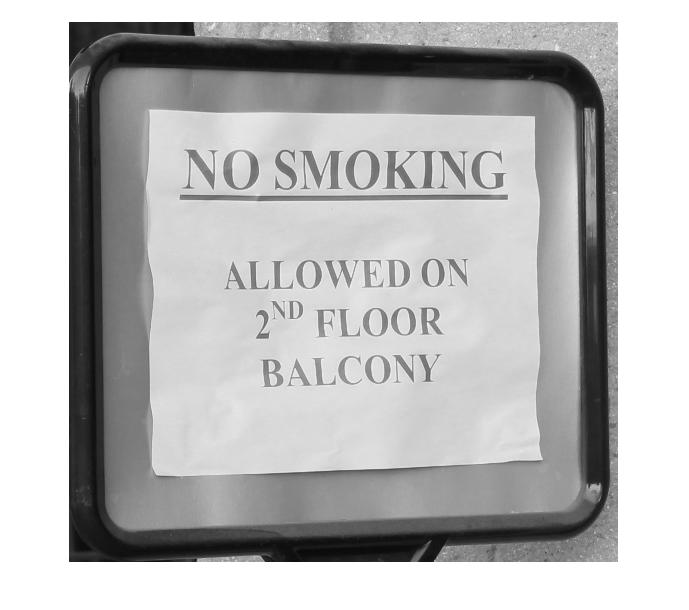
\includegraphics[width=\textwidth]{true.jpg}
                \caption{Sharp Image.\newline Grad=0.0183 ; SSI=1 ; JNB=8.4419}
               
        \end{subfigure}
        \begin{subfigure}[b]{0.3\textwidth}
                 \centering
                 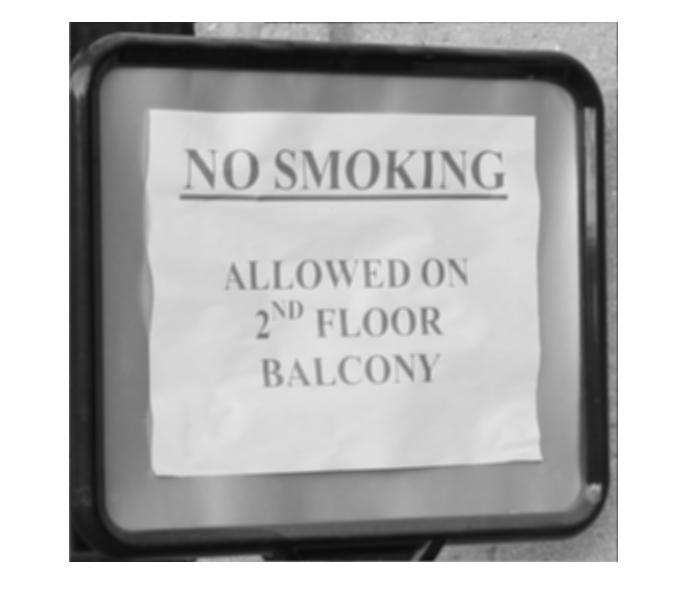
\includegraphics[width=\textwidth]{sign_D.jpg}
                 \caption{Image blurred by a disk.\newline Grad=0.0145 ; SSI=1 ; JNB=5.6732}
                       
        \end{subfigure}
        \begin{subfigure}[b]{0.3\textwidth}
                \centering
                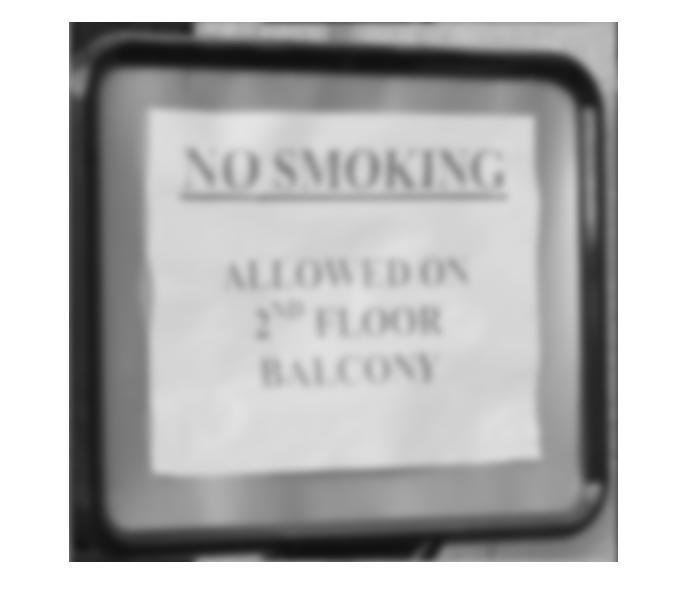
\includegraphics[width=\textwidth]{sign_G.jpg}
                \caption{Image blurred by a gaussian.\newline Grad=0.0108 ; SSI=0.9998 ; JNB=2.8083} 
        \end{subfigure} 
       
        \caption{As the blur increases in the image, the gradient value decreases, the SSI decreases and the JNB increases. The responses are independent of the blur type, and since its understood the noise levels will bias the values for some of the  coefficients, it has been ignored for this validation study.} \label{fig:train_metrics}
\end{figure}

From the study shown in Figure~\ref{fig:train_metrics}, the least reliable metric to determine sharpness is SSI, and will not be considered to be used with true images.

\subsection{True Image: Mehul}
To take advantage of the sharpness metric for real images, an automated function has been implemented in MATLAB. The function takes a blurred image and uses the metrics described above to determine which type of PSF works the best as an initial condition for the filtering process. In addition it determines which filter performs the best while sharpening the image.


\begin{figure}
        \centering
        \begin{subfigure}[b]{0.4\textwidth}
                \centering
                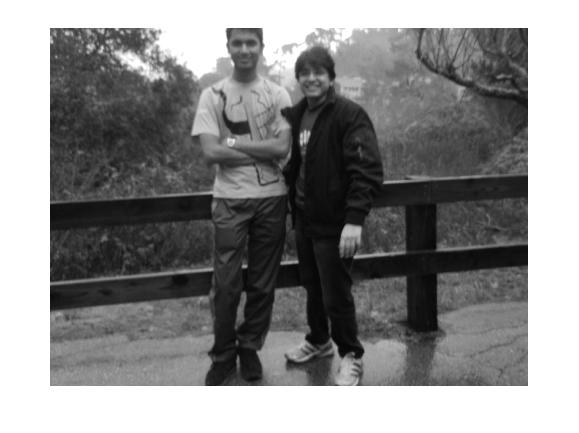
\includegraphics[width=\textwidth]{blur_personal.jpg}
                \caption{Blurry Image}
               
        \end{subfigure}
        \begin{subfigure}[b]{0.4\textwidth}
                 \centering
                 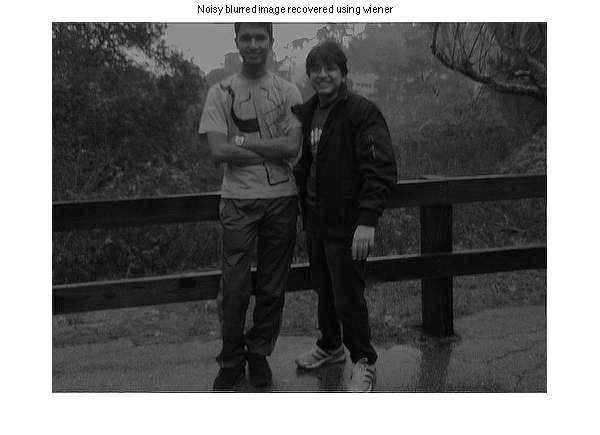
\includegraphics[width=\textwidth]{sharp_personal_bright.jpg}
                 \caption{Image sharpened by the Wiener filter }
                       
        \end{subfigure}
              
        \caption{} \label{fig:true_metrics}
\end{figure}




















%\begin{figure}
%        \centering
%        \label{fig:mehul}
%        \begin{subfigure}[b]{0.4\textwidth}
%                \centering
%                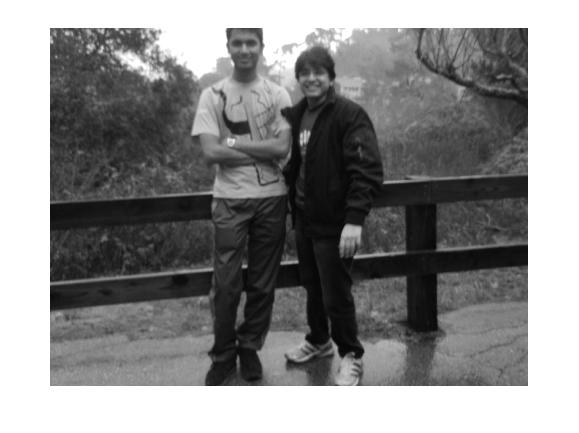
\includegraphics[width=\textwidth]{blur_personal.jpg}
%                \caption{No reference blurry image}
%                
%        \end{subfigure}
%        \begin{subfigure}[b]{0.4\textwidth}
%                \centering
%                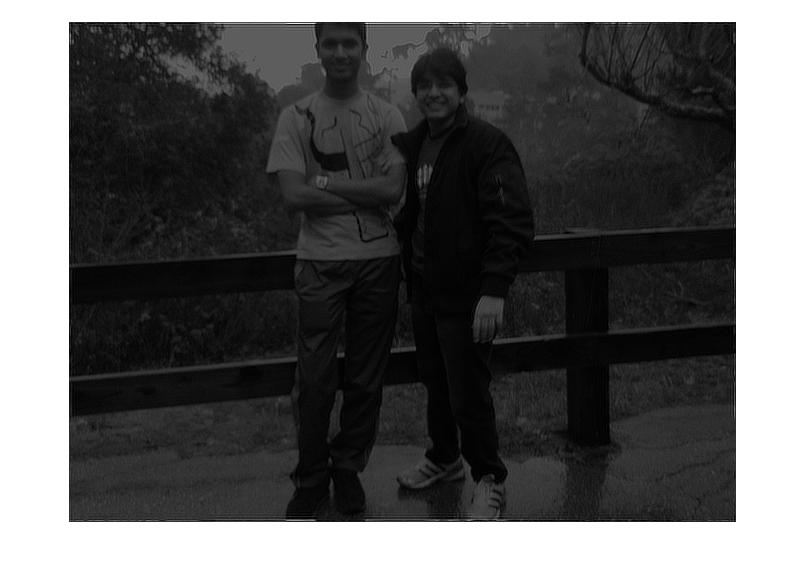
\includegraphics[width=\textwidth]{sharp_personal.jpg}
%                \caption{Wiener filter sharpened image} 
%        \end{subfigure}
%\caption{No reference image enhancement}
%\end{figure}



\newpage